\subsection{Operation flow}

Firstly, all variables used for PID, IMU, and flash memory are declared. If the drone is attached to a serial monitor, it will enter debug mode. If the user enters the character “i” on the serial monitor while in debug mode, the quadcopter will display all of the flash memory data, including previously recorded data and the memory's state. 
If the user enters the character "d", the memory is cleaned, as are the residual pointers that lead to the deleted memory (garbage collection). If the quadcopter was not previously attached to a serial monitor before entering debug mode, it would enter flying mode. 
To counteract the current spike, the motors will ramp up after recieving a BLE signal. The quadcopter will thereafter enter the control loop as long as there was no BLE signal recieved. Additionally, if the value of "time" is less than the value of "set time." The IMU and IR measurements are recorded in the control loop after being sent to the complementary filter. The current Z, $\phi$/roll, and $\theta$/pitch are all sent to their individual PID controllers, where the error is determined using the previously defined PID values. 
The errors are transformed into a specific motion that should be accomplished using the motion equations (See Chapter \ref{plant_eq}) 
As the output is still an angular velocity, it gets converted to PWM and saturated to be between 0 and 255 (See Figure \ref{linear}). 
The motors are then updated with their respective PWM value. 
A certain flash memory logging period is declared during initialization, and after updating the motors, a check is made to see if it is time to record the values, such as current z, $\phi$/roll, and $\theta$/pitch, for data analysis. (See chapter \ref{flash}) 
If the "set time" is exceeded, the recorded values are saved in flash memory, the motors are completely switched off, and the code terminates execution.

\begin{figure}[!ht]
    \begin{center}
    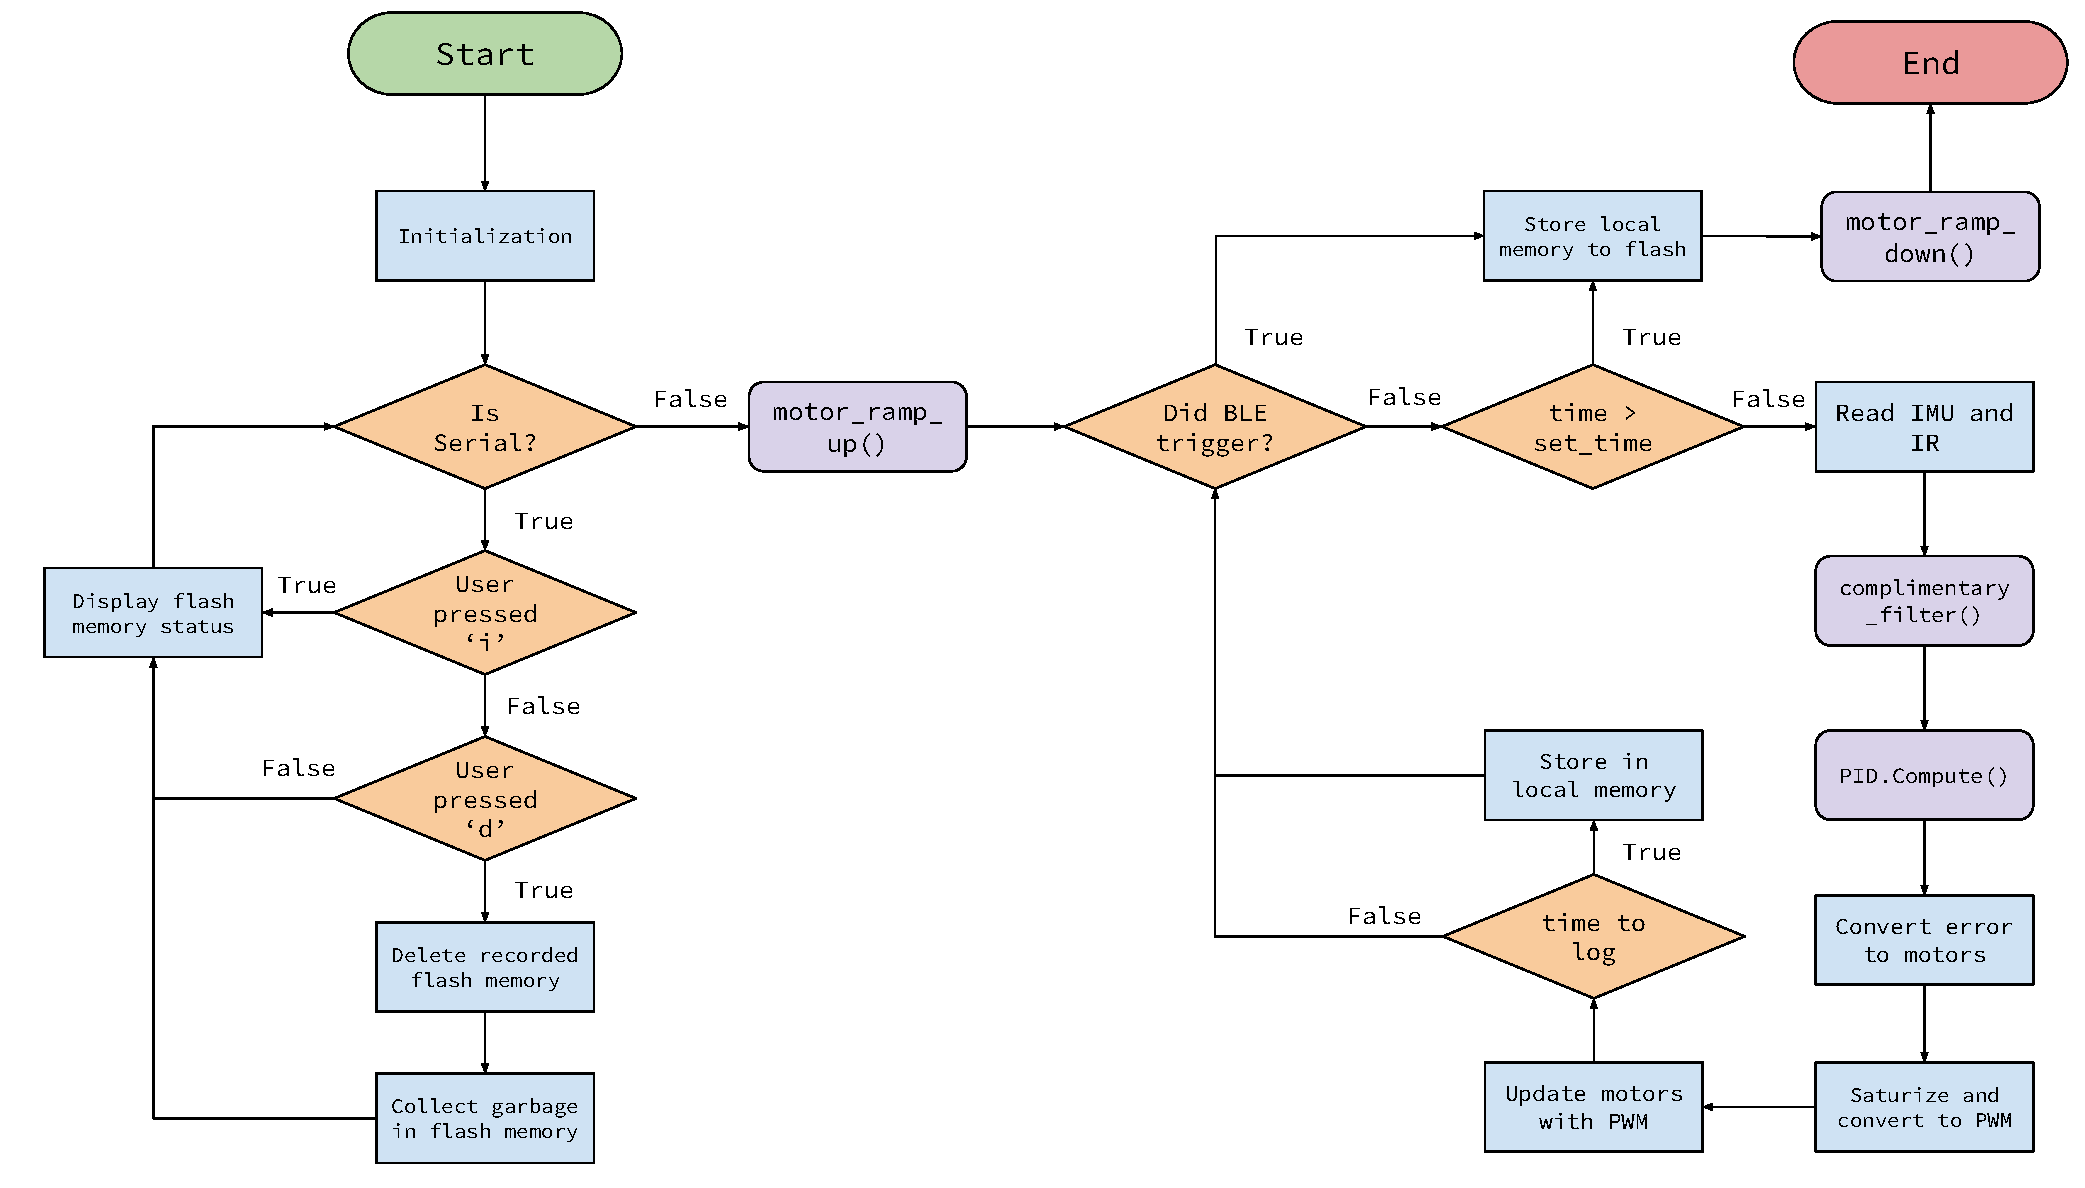
\includegraphics[width=\textwidth]{pictures/flowchart_pdf.pdf}
    \end{center}
    \caption{Flowchart describing the operation flow}
    \label{fig:flowchart}
\end{figure}